\documentclass[runningheads]{llncs}
\usepackage[T1]{fontenc}
\usepackage{graphicx}
\usepackage{subfigure}

\begin{document}
%
\title{Problema de las 8 reinas. 2 Propuestas de solución}
\author{Angel García Báez \inst{1}}
%
\institute{Universidad Veracruzana. Instituto de Investigaciones en Inteligencia Artificial}
\maketitle              % typeset the header of the contribution
%
%
%
\section{Detalles de las implementaciones}

Para resolver el problema de las 8 reinas, se propusieron 2 algoritmos genéticos que se diferencian principalmente por su representación del problema. El primer algoritmo se caracteriza por ser "ingenuo" y usar la representación de tuplas, genera soluciones aleatorias del problema bajo la restricción de que no ponga a 2 reinas en la misma posición.
 El segundo algoritmo se caracteriza por usar la representación de las permutaciones y estar "informado" debido a que coloca una reina por cada fila del tablero.

La siguiente tabla muestra las especificaciones resumidas de cada uno de los algoritmos implementados.

\begin{table}
	\caption{Parámetros de los Algoritmos Genéticos}\label{tab3}
	\begin{tabular}{|l|l|l|}
		\hline
		Parámetros & Algoritmo 1 & Algoritmo 2 \\
		\hline
		Representación & Tuplas/Listas & Permutaciones \\
		\hline
		Recombinación & Cruce de un punto & Cortar-y-llenar-cruzado \\
		\hline
		Probabilidad de recombinación & 50\% & 100\% \\
		\hline
		Mutación & Intercambio de coordenada & Intercambio (swap) \\
		\hline
		Probabilidad de mutación & 30\% & 80\% \\
		\hline
		Selección de padres & Ruleta ponderada & Best-two out of 5 random \\
		\hline
		Reemplazo & Replace-worst & Replace-worst \\
		\hline
		Tamaño de población & 100 & 100 \\
		\hline
		Número de descendientes & 50 & 2 \\
		\hline
		Inicialización & Random & Random \\
		\hline
		Condición de paro & Solución o 10,000 evaluaciones & Solución o 10,000 evaluaciones \\
		\hline
	\end{tabular}
\end{table}

La selección de parámetros se calibró de manera que para el algoritmo 1 se mantuvieron los valores propuestos en clase, mientras que para el algoritmo 2 los parámetros inicialmente recomendados arrojaron buenos resultados, por lo que no fue necesario modificarlos.

Se realizaron 30 corridas aleatorias para cada algoritmo deacuerdo con las especificaciones de la tabla 1. En cada corrida se fueron guardando los resultados de la generación, el numero de ataques y el número de evaluaciones para poder hacer estadísticas en la siguiente sección.

\section{Resultados}

\vspace{-10pt}  % Reducir el espacio entre la tabla y la figura


\begin{table}[htbp]
	\centering
	\caption{Comparativa de resultados entre algoritmos}
	\begin{tabular}{|c|cc|cc|}
		\hline
		& \multicolumn{2}{c|}{\textbf{No. de Ataques NO exitosos }} & \multicolumn{2}{c|}{\textbf{No. de Evaluaciones exitosos }} \\
		\cline{2-5}
		\textbf{Estadísticas} & \textbf{Tuplas (30)} & \textbf{Permutaciones (0)} & \textbf{Tuplas (0)} & \textbf{Permutaciones (30)} \\
		\hline
		Mejor & 2 & 0 & 10000 & 100 \\
		Media & 3.77 & 0 & 10000 & 218.6 \\
		Mediana & 4 & 0 & 10000 & 162 \\
		Desviación & 0.73 & 0 & 0 & 128.45 \\
		Peor & 5 & 0 & 10000 & 506 \\
		\hline
	\end{tabular}
	\label{tab:comparativa_algoritmos}
\end{table}

\vspace{-30pt}  % Reducir el espacio entre la tabla y la figura


\begin{figure}[htbp]
	\centering
	\subfigure[Convergencia de los ataques representación de Tuplas.]{
		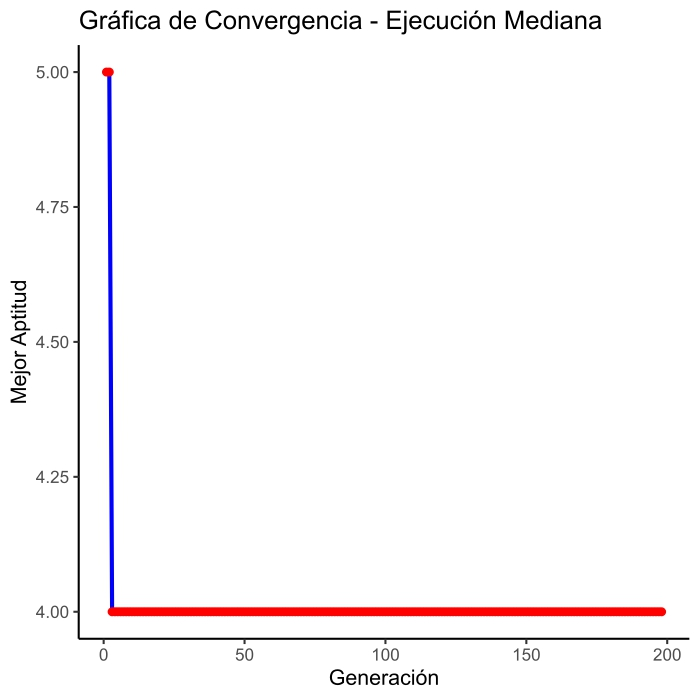
\includegraphics[width=0.45\textwidth]{M2.jpg}
		\label{fig:M2}
	}
	\hfill
	\subfigure[Convergencia de las evaluaciones representación de permutaciones.]{
		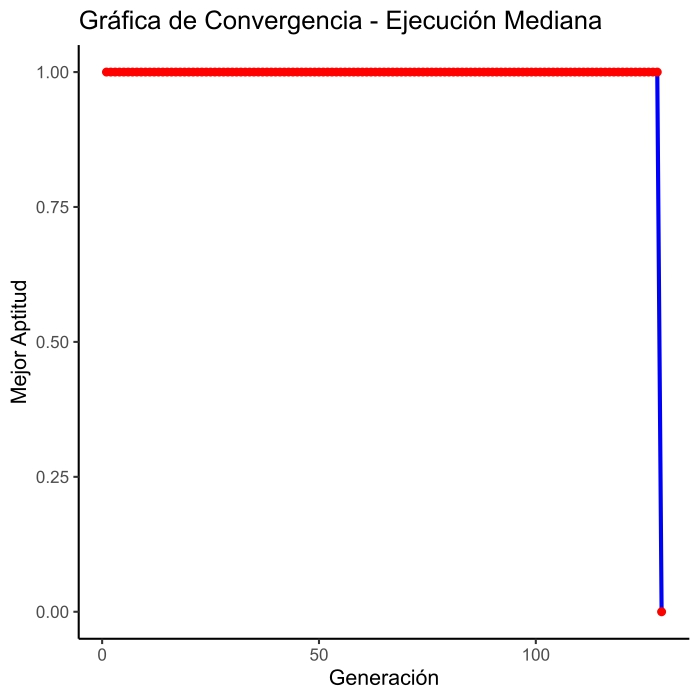
\includegraphics[width=0.45\textwidth]{M1.jpg}
		\label{fig:M1}
	}
	\caption{Comparativa de la convergencia de los ataques entre el algoritmo 1 y el algoritmo 2.}
	\label{fig:modelos}
\end{figure}

\section{Discusión de resultados}

Los resultados demuestran que la representación de permutaciones presenta un mejor desempeño en comparación con la representación de tuplas . Este rendimiento superior se fundamenta en la información inherente a la representación de permutaciones, la cual facilita la generación de soluciones que descartan alternativas no deseadas. De este modo, se restringe el espacio de soluciones a aquellas donde existe una única reina por fila (o columna).  Este comportamiento se refleja en los resultados, donde se alcanza una convergencia media en 218 evaluaciones, con una desviación estándar de 128 evaluaciones.  La representación con tuplas llega al limite permitido de evaluaciones sin converger. La mejor solución encontrada por este algoritmo presentó, como máximo, 2 ataques, y la mediana de las soluciones en 4. 


\end{document}
